\documentclass[11pt,a4paper]{article}

% ---------------------------------------------------------------------------
%  Detecting and quantifying spatial information leakage in predictive
%  modelling: a diagnostic framework and the spLeakage R package
% ---------------------------------------------------------------------------

\usepackage[utf8]{inputenc}
\usepackage[T1]{fontenc}
\usepackage{lmodern}
\usepackage[a4paper,margin=2.5cm]{geometry}
\usepackage{amsmath,amssymb,amsthm}
\usepackage{bm}
\usepackage{graphicx}
\usepackage{booktabs}
\usepackage{array}
\usepackage{caption}
\usepackage{subcaption}
\usepackage{xcolor}
\usepackage[hidelinks]{hyperref}
\usepackage{url}
\usepackage{natbib}
\usepackage{authblk}
\usepackage{setspace}
\usepackage{enumitem}
\usepackage{microtype}
\usepackage{listings}

\bibliographystyle{apalike}

% line numbers for review
\usepackage{lineno}

% --- listings style for R code ---
\definecolor{codegray}{gray}{0.95}
\lstset{
  basicstyle=\ttfamily\footnotesize,
  backgroundcolor=\color{codegray},
  breaklines=true,
  frame=single,
  framesep=4pt,
  rulecolor=\color{black!25},
  keepspaces=true,
  columns=fullflexible,
  language=R,
  showstringspaces=false
}

\newtheorem{proposition}{Proposition}
\newtheorem{definition}{Definition}

\newcommand{\SLI}{\mathrm{SLI}}
\newcommand{\SLIrho}{\SLI_{\rho}}
\newcommand{\SLId}{\SLI_{d}}
\newcommand{\EV}{\mathrm{EV}}
\newcommand{\E}{\mathbb{E}}
\newcommand{\Var}{\mathrm{Var}}
\newcommand{\cor}{\mathrm{cor}}
\newcommand{\Gobs}{\widehat{G}_{\mathrm{obs}}}
\newcommand{\Gpred}{\widehat{G}_{\mathrm{pred}}}

\title{\bfseries Detecting and quantifying spatial information leakage in
predictive modelling: a diagnostic framework and the \texttt{spLeakage}
R~package}

\author[1]{Olatunji Johnson}
\affil[1]{Department of Mathematics, University of Manchester, Manchester, UK\\
\texttt{olatunji.johnson@manchester.ac.uk}}

\date{\today}

\begin{document}

\maketitle
\linenumbers

% ===========================================================================
\begin{abstract}
\noindent
Spatial predictive models---in disease mapping, species distribution modelling,
digital soil mapping and remote sensing---routinely report accuracy estimated by
random cross-validation (CV). When observations are spatially autocorrelated,
training and test points that fall close together share information, so the
reported error measures near-interpolation rather than the out-of-sample
prediction the map is actually used for. The resulting accuracy is
\emph{optimistically biased}. A family of spatially corrected CV schemes exists to
\emph{prevent} this, but they \emph{generate folds}; none takes a split a user has
\emph{already} made and reports how much it leaks or how inflated the numbers are.
The field is moreover split by a live controversy: nearest-neighbour-matching CV
(NNDM/kNNDM) argues CV geometry must imitate prediction geometry, whereas
design-based critics argue that for probability samples random CV is unbiased and
spatial CV is \emph{pessimistic}.
We resolve both problems with a single thesis: \textbf{spatial leakage and
optimism are only well-posed relative to a declared
design~$\times$~estimand~$\times$~target}, and the same split can be leaking,
correct, or pessimistic depending on those declarations. Under this framing we
(i) give optimism a formal estimand---excess explained variance under a Gaussian
process---together with a closed-form nearest-neighbour expression and a
Wasserstein-1 bound; (ii) define a \emph{signed} Spatial Leakage Index (SLI) that
audits any split post-hoc and decomposes leakage to folds and points; (iii)
quantify optimism through a refit-free, simulation-calibrated emulator that carries
its own area-of-applicability guard; and (iv) turn the controversy into an
estimand-first recommendation engine. Across exact Gaussian-process algebra the SLI
is a near-sufficient statistic for true optimism ($r=0.98$), the signed index
predicts \emph{signed} optimism where NNDM's unsigned statistic cannot
($r=0.98$ vs $-0.09$), and the emulator attains held-out $R^2\approx0.76$ with
$\approx94\%$ interval coverage. A 16-dataset meta-audit finds reported accuracy
optimistic in \textbf{100\%} of cases (median 22\%), and reveals that optimism
decomposes into an autocorrelation channel (which spatial CV diagnoses) and a
trend-extrapolation channel (which it misses). All methods are implemented in the
open-source \texttt{spLeakage} R package, which audits rather than generates folds
and interoperates with the established spatial-CV ecosystem.
\end{abstract}

\noindent\textbf{Keywords:} spatial cross-validation; map accuracy; information
leakage; optimism; area of applicability; Gaussian process; distribution shift;
disease mapping; species distribution models; reproducibility.

\bigskip
\onehalfspacing

% ===========================================================================
\section{Introduction}\label{sec:intro}

Maps produced by statistical and machine-learning models underpin decisions in
public health, conservation, agriculture and earth observation. The credibility of
such a map rests almost entirely on a single reported number---its estimated
predictive accuracy. Yet for spatial data this number is systematically
unreliable. Observations collected over space are autocorrelated: nearby locations
have similar values. When a model is validated by an ordinary random train/test
split, test points routinely have a training neighbour only a short distance
away. The model is therefore evaluated on a task close to \emph{interpolation},
whereas at deployment it must predict at locations far from any training data. The
reported error understates the true error: it is \emph{optimistically biased}, an
instance of \emph{information leakage} from training to test \citep{roberts2017crossvalidation,
ploton2020spatial, kattenborn2022spatially}.

The consequences are not academic. \citet{ploton2020spatial} showed in
\emph{Nature Communications} that large-scale ecological maps are far less accurate
than reported once spatial structure is respected. The same overconfidence has been
documented for convolutional networks on remote-sensing imagery
\citep{kattenborn2022spatially} and is a recurring concern in species distribution
modelling and digital soil mapping. A decision-maker who trusts an inflated
accuracy figure will over-rely on a map that is, in the regions that matter most
(those far from data), much weaker than advertised.

\paragraph{The methodological response, and its gap.}
A mature family of \emph{spatially aware} cross-validation methods exists to avoid
the problem by constructing better folds: spatial block CV
\citep{roberts2017crossvalidation, valavi2019blockcv}, buffered / spatial
leave-one-out CV \citep{lerest2014sloo, telford2009evaluation}, and
nearest-neighbour distance matching CV \citep[NNDM/kNNDM;][]{mila2022nndm,
linnenbrink2024knndm}, packaged in tools such as \texttt{CAST}
\citep{meyer2024cast}, \texttt{blockCV} \citep{valavi2019blockcv},
\texttt{spatialsample} and \texttt{sperrorest} \citep{brenning2012sperrorest}.
These are \emph{fold generators}. They answer ``how should I cross-validate?''.
None of them answers the question a practitioner who has already run an analysis
actually asks: \emph{``I already have a split (or a published result). How much does
it leak, and how inflated is my reported accuracy?''} There is no leakage
\emph{diagnostic}, no \emph{audit}, and no \emph{optimism estimate} for an arbitrary
split. This is the gap \texttt{spLeakage} fills.

\paragraph{A live controversy.}
Worse, the field disagrees about what ``correct'' validation even is.
\citet{mila2022nndm} and \citet{linnenbrink2024knndm} argue that the CV geometry
should match the prediction geometry, making random CV optimistic for clustered
data. \citet{wadoux2021spatial} argue, from a design-based standpoint, that
``spatial cross-validation is not the right way to evaluate map accuracy'': for a
\emph{probability sample}, random validation is design-unbiased and spatial CV
introduces a \emph{pessimistic} bias \citep[see also][]{debruin2022clustered}.
\textbf{Both camps are right---in different regimes.} A practitioner has no tool
that tells them which regime they are in, and therefore which validation is
correct.

\paragraph{Our contribution.}
We argue that the gap and the controversy have a common root and a common
resolution. Spatial leakage and optimism are \emph{not} properties of a dataset or
a split in isolation; they are only well-defined \emph{relative to a declared
sampling design, a declared estimand, and a declared prediction target}
(Section~\ref{sec:thesis}). The same split can be leaking, correct, or pessimistic
according to these three declarations. Making them explicit (i) dissolves the
Mil\`a--Wadoux controversy---each side is correct in a different cell of the
design~$\times$~estimand~$\times$~target space---and (ii) removes a circular
dependency that would otherwise undermine any optimism estimate. On this
foundation we build four contributions:

\begin{enumerate}[leftmargin=1.4em,itemsep=2pt]
\item \textbf{A formal estimand and theory for optimism}
  (Section~\ref{sec:theory}). Under a Gaussian process, optimism equals the
  \emph{excess explained variance} a CV scheme enjoys over deployment; this yields a
  closed-form nearest-neighbour expression and a Wasserstein-1 bound that connect
  spatial leakage to distribution-shift generalization theory.
\item \textbf{A signed Spatial Leakage Index (SLI)}
  (Section~\ref{sec:sli}): a post-hoc, dependence-aware, \emph{signed} leakage score
  for any split, with a decomposition to folds and points (a leakage map) that
  fold-generators cannot produce.
\item \textbf{A refit-free optimism estimator}
  (Section~\ref{sec:optimism}): an empirical route and a simulation-calibrated
  emulator with adaptive predictive intervals and its own area-of-applicability
  guard---``your reported error is $X\%$ optimistic ($a$--$b\%$)''.
\item \textbf{A design-aware recommendation and correction layer}
  (Section~\ref{sec:recommend}): an estimand-first decision engine, a de-leaked
  accuracy estimate that can correct a \emph{published} number without refitting,
  and an optimal design for \emph{validation} survey placement.
\end{enumerate}

Every method is implemented in the open-source \texttt{spLeakage} R package
(Section~\ref{sec:software}), which \emph{audits rather than generates} folds and
interoperates with \texttt{CAST}, \texttt{blockCV}, \texttt{spatialsample} and
\texttt{mlr3spatiotempcv}. Section~\ref{sec:results} validates every claim with
exact Gaussian-process algebra, a head-to-head benchmark against NNDM, an
out-of-sample emulator study, independent real-data validation, a 16-dataset
meta-audit, and two real case studies (a species distribution model and a malaria
prevalence map). Section~\ref{sec:discussion} discusses scope,
limitations and the new two-channel decomposition of optimism that the meta-audit
reveals.

% ===========================================================================
\section{Leakage is well-posed only relative to design, estimand and
target}\label{sec:thesis}

The central claim of the paper is a reframing:

\begin{quote}\itshape
``Spatial leakage'' and ``optimism'' are not properties of a dataset or a split in
isolation. They are well-defined only relative to a declared sampling
\textbf{design}, a declared \textbf{estimand}, and a declared prediction
\textbf{target}. The same split can be leaking, correct, or pessimistic depending
on these three declarations.
\end{quote}

\noindent The three declarations play distinct roles.

\begin{description}[leftmargin=0pt,itemsep=3pt]
\item[Sampling design.] Whether the data are a probability sample (with known
  inclusion probabilities), a designed cluster sample, or a convenience sample
  decides whether random validation is unbiased \citep{wadoux2021spatial,
  debruin2022clustered} or optimistic \citep{mila2022nndm}. Crucially,
  design-basedness is a fact about \emph{how the data were collected}; it cannot be
  recovered from the coordinates. A designed cluster sample and a convenience
  sample can produce identical point patterns. Geometry (Clark--Evans index,
  Ripley's $K$) can therefore only \emph{flag risk}; the design is an
  \emph{elicited input}, never an inference.
\item[Estimand.] \emph{Population-mean map accuracy over a region} (a design-based
  quantity) and \emph{conditional predictive skill at a location} (a model-based
  quantity) are different questions. Conflating them is a common error and a
  frequent reviewer objection. We separate them and never recommend a validation
  scheme \emph{across} estimands.
\item[Prediction target.] Within-sample interpolation, wall-to-wall mapping, and
  new-region extrapolation imply different deployment geometries, and hence
  different ``correct'' validation geometries.
\end{description}

This reframing is what makes ``optimism'' computable. We define optimism not
against NNDM-as-truth, but against \emph{the validation that is correct for the
declared design~$\times$~estimand~$\times$~target}. For a probability sample with a
population-mean estimand, the correct baseline is design-based/random validation,
so a spatially blocked scheme registers as \emph{pessimism} (negative optimism)---
exactly the Wadoux case, now reported as such rather than hidden. The declarations
are inputs, not inferences, which is what removes the circularity that would
otherwise make the optimism estimate ill-posed. The reconciliation of the
controversy is, in this sense, the paper's primary intellectual contribution; the
index, the emulator and the recommender are its instantiations.

% ===========================================================================
\section{Theory: optimism as a distribution-shift gap}\label{sec:theory}

We now give optimism a formal estimand and show that a simple geometric index is
its leading term. This converts the SLI from a validated heuristic into a
principled method and connects spatial leakage to distribution-shift theory.

\subsection{Model and the explained-variance estimand}

Let $Z$ be a zero-mean Gaussian process with stationary covariance
$\mathrm{Cov}(Z(s),Z(s'))=\sigma^2\rho(\lVert s-s'\rVert)$, observed with
independent nugget noise,
\begin{equation}
Y(s)=\mu+Z(s)+\varepsilon(s),\qquad \varepsilon\sim N(0,\tau^2),\quad
\varepsilon \perp Z .
\end{equation}
Write the total variance $V=\sigma^2+\tau^2$ and the \emph{signal proportion}
$w=\sigma^2/V\in[0,1]$. Simple kriging of $Y(s_0)$ from a training set $T$ of $m$
observations has mean-squared error
\begin{equation}\label{eq:mse}
\mathrm{MSE}(s_0\mid T)=V - c_0^\top \Sigma^{-1} c_0 ,
\qquad c_0=\sigma^2\rho(s_0,T),\ \ \Sigma=\sigma^2 R + \tau^2 I,
\end{equation}
where $R$ is the correlation matrix of $T$. Call
$\EV(s_0\mid T)=c_0^\top\Sigma^{-1}c_0\ge 0$ the \emph{explained variance}: the
reduction in predictive variance the training data contributes, large when $s_0$ is
near (correlated with) the training points, small when far.

A CV scheme predicts each test point $t$ from its fold's training set $\mathrm{Tr}(t)$;
deployment predicts each target location $p$ from the full sample $S$. Averaging
\eqref{eq:mse}, the constant $V$ cancels and the optimism---the gap between the true
deployment error $E_{\text{true}}$ and the cross-validated error $E_{\text{cv}}$---is

\begin{equation}\label{eq:optimism}
\text{optimism}=E_{\text{true}}-E_{\text{cv}}
=\underbrace{\tfrac1n\textstyle\sum_t \EV(t\mid \mathrm{Tr}(t))}_{\text{CV explains}}
-\underbrace{\tfrac1m\textstyle\sum_p \EV(p\mid S)}_{\text{deployment explains}} .
\end{equation}

\begin{proposition}[Optimism is excess explained variance]
Equation~\eqref{eq:optimism} holds for \emph{any} Gaussian process, with no
approximation. Optimism is exactly the excess explained variance that the CV scheme
enjoys over deployment.
\end{proposition}

\noindent This is the formal estimand: an interpretable population quantity, not a
heuristic. It also makes the sign meaningful---optimism is positive when CV is
``easier'' than deployment and negative (pessimism) when CV is harder, the Wadoux
regime.

\subsection{The nearest-neighbour closed form and where the SLI appears}

Keeping only the nearest training point, at distance $d$, gives
$c_0=\sigma^2\rho(d)$, $\Sigma=V$, and hence the pointwise loss
\begin{equation}\label{eq:Ld}
L(d)=\mathrm{MSE}\approx V\bigl[\,1-w^2\rho(d)^2\,\bigr].
\end{equation}
Substituting into \eqref{eq:optimism}, with $g$ the test$\to$train and $f$ the
deployment$\to$sample nearest-neighbour distances,
\begin{equation}\label{eq:sliform}
\text{optimism}\approx V\,w^2\Bigl(\E_t[\rho(g)^2]-\E_p[\rho(f)^2]\Bigr).
\end{equation}
Equation~\eqref{eq:sliform} is, up to the scale $Vw^2$, exactly a difference of mean
retained spatial correlation between CV and deployment---the Spatial Leakage Index
of Section~\ref{sec:sli}. The theory therefore predicts \emph{which} features govern
optimism: the correlation function $\rho$ (hence range and smoothness), the signal
proportion $w$, and the nearest-neighbour-distance laws of the split and the
target. These are precisely the inputs of the emulator
(Section~\ref{sec:optimism}); the emulator was empirically rediscovering
\eqref{eq:sliform}.

\subsection{A Wasserstein bound}

Let $P_{\text{cv}}$ and $P_{\text{dep}}$ be the laws of the test$\to$train and
deployment$\to$sample nearest-neighbour distances. By \eqref{eq:Ld},
\begin{equation}
\text{optimism}\approx \int L\, d(P_{\text{dep}}-P_{\text{cv}}),
\end{equation}
a distribution-shift generalization gap: the same loss $L$ under two laws of the
governing distance. Because $L$ is bounded-Lipschitz, the
Kantorovich--Rubinstein duality \citep{villani2009optimal} gives
\begin{equation}\label{eq:wbound}
\lvert\text{optimism}\rvert \le \lVert L'\rVert_\infty\, W_1(P_{\text{cv}},P_{\text{dep}}),
\end{equation}
where $W_1$ is the Wasserstein-1 distance between the two ECDFs---which is, up to the
range normalisation, the distance-form index $\SLId$. Thus $\SLIrho$ gives the
optimism \emph{value} \eqref{eq:sliform} and $\SLId$ gives a rigorous \emph{bound}
\eqref{eq:wbound}. This framing also imports the distribution-shift toolkit
(importance weighting, integral-probability-metric bounds) as a route to
model-agnostic optimism bounds beyond the Gaussian case. Scope and the
multi-neighbour correction are discussed in Section~\ref{sec:discussion}; numerical
validation is in Section~\ref{sec:res-theory}.

% ===========================================================================
\section{The signed Spatial Leakage Index}\label{sec:sli}

\subsection{Construction}

For a split, let $g_{\text{obs}}(t)=\min_{s\in\mathrm{Tr}(t)} d(t,s)$ be the
test$\to$train nearest-neighbour distance and $f_{\text{pred}}(p)=\min_{s\in S}
d(p,s)$ the deployment$\to$sample distance, where $d$ is geodesic for geographic
coordinate reference systems and projected otherwise. Their ECDFs are $\Gobs$ and
$\Gpred$. Leakage means test points are \emph{closer} to their training data during
CV than deployment points are to the sample, i.e.\ $\Gobs$ is shifted to smaller
distances than $\Gpred$.

\paragraph{Distance form.} The signed area between the ECDFs,
\begin{equation}
A=\int_0^\infty\!\bigl(\Gobs(r)-\Gpred(r)\bigr)dr
 = \E_p[f_{\text{pred}}]-\E_t[g_{\text{obs}}],
\end{equation}
is literally how much farther deployment reaches than CV pretended, in distance
units. Normalising by the variogram practical range $\varphi$ (the intrinsic
dependence length, \emph{not} the map extent, which gives cross-dataset invariance)
yields $\SLId=A/\varphi$. To prevent cancellation when the ECDFs cross (leakage at
short range, pessimism at long range) we report the crossing decomposition
$A_+=\int\max(\Gobs-\Gpred,0)$, $A_-=\int\max(\Gpred-\Gobs,0)$, $A=A_+-A_-$, and
$W=A_++A_-$. Here $W$ is exactly the unsigned NNDM/kNNDM Wasserstein statistic, so
$\SLId$ reduces to $W$ in magnitude when the ECDFs do not cross---the explicit
bridge to the established literature. The directionality ratio
$\delta=A/W\in[-1,1]$ flags whether a single number is trustworthy ($\delta\approx
\pm 1$) or the user should inspect the ECDF plot ($\delta\approx 0$).

\paragraph{Dependence form (headline).} Because geographic distance is not
statistical dependence, we replace raw distances by the fitted spatial correlation
$\rho(h)$ and define the retained spatial information
\begin{equation}
c_{\text{obs}}=\tfrac1n\textstyle\sum_t\rho(g_{\text{obs}}(t)),\quad
c_{\text{pred}}=\tfrac1m\textstyle\sum_p\rho(f_{\text{pred}}(p)),\quad
\boxed{\ \SLIrho=c_{\text{obs}}-c_{\text{pred}}\in[-1,1].\ }
\end{equation}
$\SLIrho$ is bounded, dimensionless and signed: $+$ means CV retains more spatial
information than deployment has (optimistic leakage), $-$ means pessimism. Under
anisotropy or non-stationarity a directional/local $\rho$ is used, so the index
tracks \emph{dependence} rather than geometry. By
Section~\ref{sec:theory}, $\SLIrho$ is the leading term of true optimism
(scaled by $Vw^2$), which is what validates the index.

\subsection{Decomposition: the leakage map}

The per-observation contribution $\ell(t)=\rho(g_{\text{obs}}(t))-c_{\text{pred}}$
satisfies $\SLIrho=\tfrac1n\sum_t\ell(t)$. Mapping $\ell(t)$ over space shows
\emph{where} a split leaks; averaging within folds shows \emph{which} folds leak.
This per-point/per-fold decomposition of an arbitrary split is the substantive
contribution of the index---it is exactly what a fold-generator cannot produce.

\subsection{Why this is not ``NNDM's \texorpdfstring{$W$}{W} renamed''}

The contribution is the \emph{signing}, the \emph{decomposition}, and the
\emph{post-hoc audit of an arbitrary split}, not the underlying ECDF comparison.
NNDM constructs folds to minimise $W$; the SLI takes any split and reports a signed,
dependence-aware, mappable diagnostic. Section~\ref{sec:res-benchmark} shows
quantitatively that the unsigned $W$ cannot recover the sign of optimism, whereas
the signed SLI can.

\subsection{Uncertainty}

$\varphi$ and $\rho$ are estimated, often from the very clustered data that leaks.
The default is a plug-in SLI from a fitted variogram; optionally, variogram
parameters are sampled from their uncertainty and the SLI is recomputed per draw,
giving a Monte-Carlo interval whose coverage is checked in simulation.

% ===========================================================================
\section{Quantifying optimism}\label{sec:optimism}

The SLI says \emph{whether} and \emph{in which direction} a split leaks. The
practitioner wants the number in their own currency: ``my reported RMSE is $X\%$
optimistic''. We provide two routes.

\paragraph{(a) Empirical route.} Re-evaluate the user's model under the
\emph{design-matched correct} scheme (block or buffered-block CV for the clustered
case) and report the gap to the user's scheme. This is accurate but
model-conditional and requires refits; it is reported as model-conditional and can
be negative (pessimism). It is implemented model-agnostically via a pluggable
prediction function (inverse-distance weighting by default).

\paragraph{(b) Emulator route (refit-free).} A pre-trained predictor maps
$(\text{range},\ \text{smoothness},\ \text{signal } w,\ \text{sample size } n,\
\text{clustering},\ \SLIrho,\ \text{design},\ \text{target})\mapsto$ expected
optimism, calibrated once by a large simulation study shipped with the package and
applied instantly with no refitting. The generator is deliberately rich: Mat\'ern
fields across smoothness $\{0.5,1.5,2.5\}\times$ signal $\times$ \{random,
clustered (varied tightness), preferential \citep{diggle2010geostatistical}\}
sampling $\times$ $n\in\{150,300,600\}$ $\times$ \{Gaussian, Poisson, Binomial\}
responses $\times$ \{IDW, random forest, GAM\} learners $\times$ \{grid,
interpolation\} targets. The point estimate is a gradient-boosted tree ensemble
\citep{chen2016xgboost}; predictive intervals are produced by
\emph{normalised split-conformal} regression \citep{vovk2005algorithmic,
romano2019conformalized}, grouped by configuration so that interval width scales
with a local difficulty estimate (the mean residual of feature-space neighbours).
Critically, the emulator carries its \emph{own} area-of-applicability check
\citep{meyer2021aoa}: queries outside the training envelope are flagged and the
estimate is withheld---the tool must not commit the sin it polices.
Section~\ref{sec:res-emulator} reports its out-of-sample performance and its correct
refusal of an out-of-distribution real-data query.

% ===========================================================================
\section{Recommendation, correction and validation design}\label{sec:recommend}

\subsection{Estimand-first recommendation}

The recommendation engine turns the thesis into actionable, \emph{conditional}
guidance. It elicits the estimand first (population-mean map accuracy vs conditional
predictive skill), then recommends over design~$\times$~target
(Table~\ref{tab:matrix}). Three rules keep it defensible: design-basedness is
\emph{elicited, never inferred from geometry}; every cell is backed by a citation or
a simulation row; and guidance is phrased conditionally (``\emph{if} your estimand
is $X$ under framework $Y$, \emph{then}\ldots''), surfacing the assumption rather
than silently adopting a side. Uncovered designs (spatiotemporal,
citizen-science, preferential intensity, multi-source fusion) are flagged and
referred, not forced into the table. Loudly, it also states \emph{when spatial CV is
not appropriate}---the nuance no current tool surfaces. A data-driven companion,
\texttt{rank\_cv\_schemes()}, builds each candidate scheme, measures its $\SLIrho$
against the declared target, and ranks by deployment match.

\begin{table}[t]
\centering
\caption{The design~$\times$~target recommendation matrix (after the estimand is
declared). Each cell is backed by a citation or a simulation-study row; the design
is an elicited input, never inferred from the point pattern.}
\label{tab:matrix}
\small
\begin{tabular}{p{3.4cm} p{3.0cm} p{3.0cm} p{3.2cm}}
\toprule
\textbf{Sampling design $\backslash$ target} & \textbf{Within-sample
interpolation} & \textbf{Wall-to-wall mapping} & \textbf{New-region
extrapolation}\\
\midrule
Probability / design-based & Random CV (design-based) & Design-based estimator &
Caution; AOA\\
Clustered / preferential & NNDM / buffered & NNDM / kNNDM & Block + AOA\\
Convenience / opportunistic & Buffered LOO & kNNDM & Block + AOA, flag risk\\
\bottomrule
\end{tabular}
\end{table}

\subsection{The de-leaked estimator}

\texttt{deleak\_estimate()} corrects a \emph{reported} accuracy value without
refitting the model, using a fold-bootstrap confidence interval. A
\texttt{target=} argument selects the control scheme whose $\SLIrho$ against the
declared target is closest to zero (NNDM matching as a selection rule). This makes
\texttt{spLeakage} a \emph{meta-audit} instrument: it can correct a published number
given only the data geometry and the reported metric
(Section~\ref{sec:res-metaaudit}).

\subsection{Optimal design for validation}

Inverting the SLI yields a survey-design tool. Given training locations, a
deployment target and a budget of $n_v$ independent validation points,
\texttt{design\_validation()} stratifies by distance-to-training on the deployment
distribution, models the per-stratum error from the GP loss $L(d)$
\eqref{eq:Ld}, and allocates the budget by Neyman allocation with Horvitz--Thompson
inclusion weights so the weighted-mean accuracy estimate stays unbiased. This is
optimal experimental design for \emph{validation} (not prediction), which the
spatial-CV literature does not address (Section~\ref{sec:res-design}).

% ===========================================================================
\section{The \texttt{spLeakage} package}\label{sec:software}

\texttt{spLeakage} is an R ($\ge 4.1$) package built on \texttt{sf}
\citep{pebesma2018sf} with all heavy adaptors (\texttt{rsample}, \texttt{mlr3},
\texttt{caret}, \texttt{blockCV}, \texttt{terra}, \texttt{gstat}) in
\texttt{Suggests} and guarded at run time. It \emph{audits rather than generates}
folds, interoperating with the spatial-CV ecosystem rather than competing with it.
The core functions are: \texttt{prediction\_target()} to declare deployment;
\texttt{detect\_leakage()} for the signed SLI; \texttt{estimate\_optimism()} and
\texttt{predict\_optimism()} for the two optimism routes;
\texttt{recommend\_validation()} and \texttt{rank\_cv\_schemes()} for guidance;
\texttt{deleak\_estimate()} for correction; \texttt{design\_validation()} for survey
design; and per-channel detectors for grouped/duplicated-location, feature-space,
temporal and trend leakage, each paired with a fix (\texttt{group\_kfold()},
\texttt{temporal\_kfold()}, design-matched controls). \texttt{audit\_workflow()}
inspects an existing resampling object and \texttt{report\_leakage()} produces a
submission-ready scorecard. All constructors return classed S3 objects with
\texttt{print}/\texttt{summary}/\texttt{plot} methods. The shipped emulator is
serialised compactly ($\approx 85$\,KB) inside the package. \texttt{R CMD check}
passes cleanly (0 errors/warnings/notes beyond the standard new-submission note).

\begin{lstlisting}[caption={A complete audit-quantify-recommend workflow.},captionpos=b]
library(spLeakage)

# 1. Declare where the model will actually be used (a wall-to-wall map)
tgt <- prediction_target(grid = pred_grid, type = "grid")

# 2. Diagnose an existing split: signed index + uncertainty + decomposition
lk <- detect_leakage(data, split = my_folds, target = tgt,
                     response = "y", n_boot = 300)
lk            # SLI_rho, 90% CI, NNDM W, signed verdict
plot(lk)      # observed-vs-deployment NN-distance ECDFs and the leakage map

# 3. Quantify the optimism it causes (refit-free emulator + empirical route)
predict_optimism(lk)
estimate_optimism(data, split = my_folds, response = "y", control = "block")

# 4. Get design-aware advice (design is declared, not inferred)
recommend_validation(data, estimand = "prediction",
                     design = "clustered", target = "grid")

# 5. Correct a reported metric without refitting
deleak_estimate(reported_rmse = 0.42, data = data,
                split = my_folds, target = tgt)
\end{lstlisting}

% ===========================================================================
\section{Results}\label{sec:results}

We validate each claim in turn: the theory (exact GP algebra), the benchmark against
NNDM, the emulator (out-of-sample), independent real-data validation, the
meta-audit, two real case studies, and the validation-design tool. Scripts to
reproduce every result ship in the package's \texttt{data-raw/} directory.

\subsection{The SLI is a near-sufficient statistic for optimism}\label{sec:res-theory}

Across 192 Gaussian-process configurations (range~$\times$~signal~$\times$~$n$
~$\times$~\{random, clustered\}), with explained variance computed \emph{exactly}
from the covariance algebra (no field realisation), the single-nearest-neighbour
closed form \eqref{eq:sliform} tracks exact optimism at $r=0.975$
(Table~\ref{tab:theory}). The package's unsquared $\SLIrho$ correlates with exact
optimism at $r=0.976$---explaining $\approx 95\%$ of the variance---and
\emph{beats} the single-NN squared form ($r=0.841$), because with realistic dense
training the explained variance saturates and the linear correlation difference is
the better sufficient statistic. The Wasserstein bound \eqref{eq:wbound} holds in
$100\%$ of configurations for the single-NN optimism it governs; the exact
multi-neighbour optimism is $\approx 1.6\times$ larger, so bounding it requires
inflating $\lVert L'\rVert$ by that factor (an honest, quantified caveat). A
$k$-neighbour extension improves magnitude but reduces correlation
(noisy-OR over-counts correlated neighbours), so $k=1$ is retained as default---a
clean negative result that vindicates the original choice.

\begin{table}[t]
\centering
\caption{Exact-GP validation of the theory (192 configurations).}
\label{tab:theory}
\small
\begin{tabular}{p{8.6cm} c}
\toprule
Claim & Result\\
\midrule
Single-NN closed form \eqref{eq:sliform} predicts exact optimism & $r=0.975$\\
$\SLIrho$ is a near-sufficient statistic for GP optimism & $r=0.976$\\
Unsquared $\SLIrho$ beats single-NN squared form & $0.976$ vs $0.841$\\
Wasserstein bound \eqref{eq:wbound} holds (single-NN optimism) & $100\%$\\
Multi-NN amplification (exact / single-NN) & median $1.56$\\
\bottomrule
\end{tabular}
\end{table}

\subsection{Signed SLI vs NNDM's unsigned \texorpdfstring{$W$}{W}}\label{sec:res-benchmark}

The natural objection---``isn't this just NNDM's $W$?''---is answered against exact
GP optimism over 288 configurations spanning
design~$\times$~split~$\times$~target~$\times$~range~$\times$~signal, of which
$64\%$ are \emph{pessimistic} (the Wadoux regime), so the test is not contrived.
The signed $\SLIrho$ predicts \emph{signed} optimism at $r=0.977$; NNDM's unsigned
$W$ at $r=-0.090$ (Table~\ref{tab:benchmark}). $W$ cannot sign the bias by
construction: a practitioner with a large $W$ does not know whether to trust their
numbers more or less. The SLI recovers the direction in $97\%$ of cases, and even on
magnitude beats $W$ ($0.955$ vs $0.672$) because $W$ is pure geometry while
$\SLIrho$ carries the signal proportion $w$ that scales optimism. NNDM solves a
fold-construction problem (make $W$ small); \texttt{spLeakage} solves a diagnosis
problem (how much, and which way, is accuracy biased).

\begin{table}[t]
\centering
\caption{Predicting exact GP optimism from the signed SLI vs NNDM's $W$
(288 configurations, 64\% pessimistic).}
\label{tab:benchmark}
\small
\begin{tabular}{l c c}
\toprule
Task & signed $\SLIrho$ & NNDM $W$ (unsigned)\\
\midrule
Predict \emph{signed} optimism & $r=+0.977$ & $r=-0.090$\\
Predict magnitude $\lvert\text{optimism}\rvert$ & $r=0.955$ & $r=0.672$\\
Direction (sign) agreement & $97\%$ & silent by construction\\
\bottomrule
\end{tabular}
\end{table}

\subsection{The emulator generalises out of sample}\label{sec:res-emulator}

On a paper-scale study (1000 configurations $\times$ 6 realisations,
$\approx 2000$ denoised rows), held out \emph{by configuration}, the emulator
attains $R^2\approx 0.76$, places $97\%$ of held-out queries inside its
area-of-applicability, and its $90\%$ predictive intervals cover at
$\approx 94\%$ (Figure~\ref{fig:calibration}). The empirical correlation
$\cor(\SLIrho,\text{optimism})=0.67$ provides direct evidence for the
SLI~$\to$~optimism mechanism (Figure~\ref{fig:sli}). The design effect that
reconciles the controversy reproduces in the data: clustered/preferential sampling
makes random CV more optimistic than a probability-like random sample, while for
well-covered grid targets random CV is fine or slightly pessimistic
(Figure~\ref{fig:design}). The \emph{ordering} is robust; the absolute level depends
on target geometry and model class, which the emulator's model-class factor
absorbs.

\begin{figure}[t]
\centering
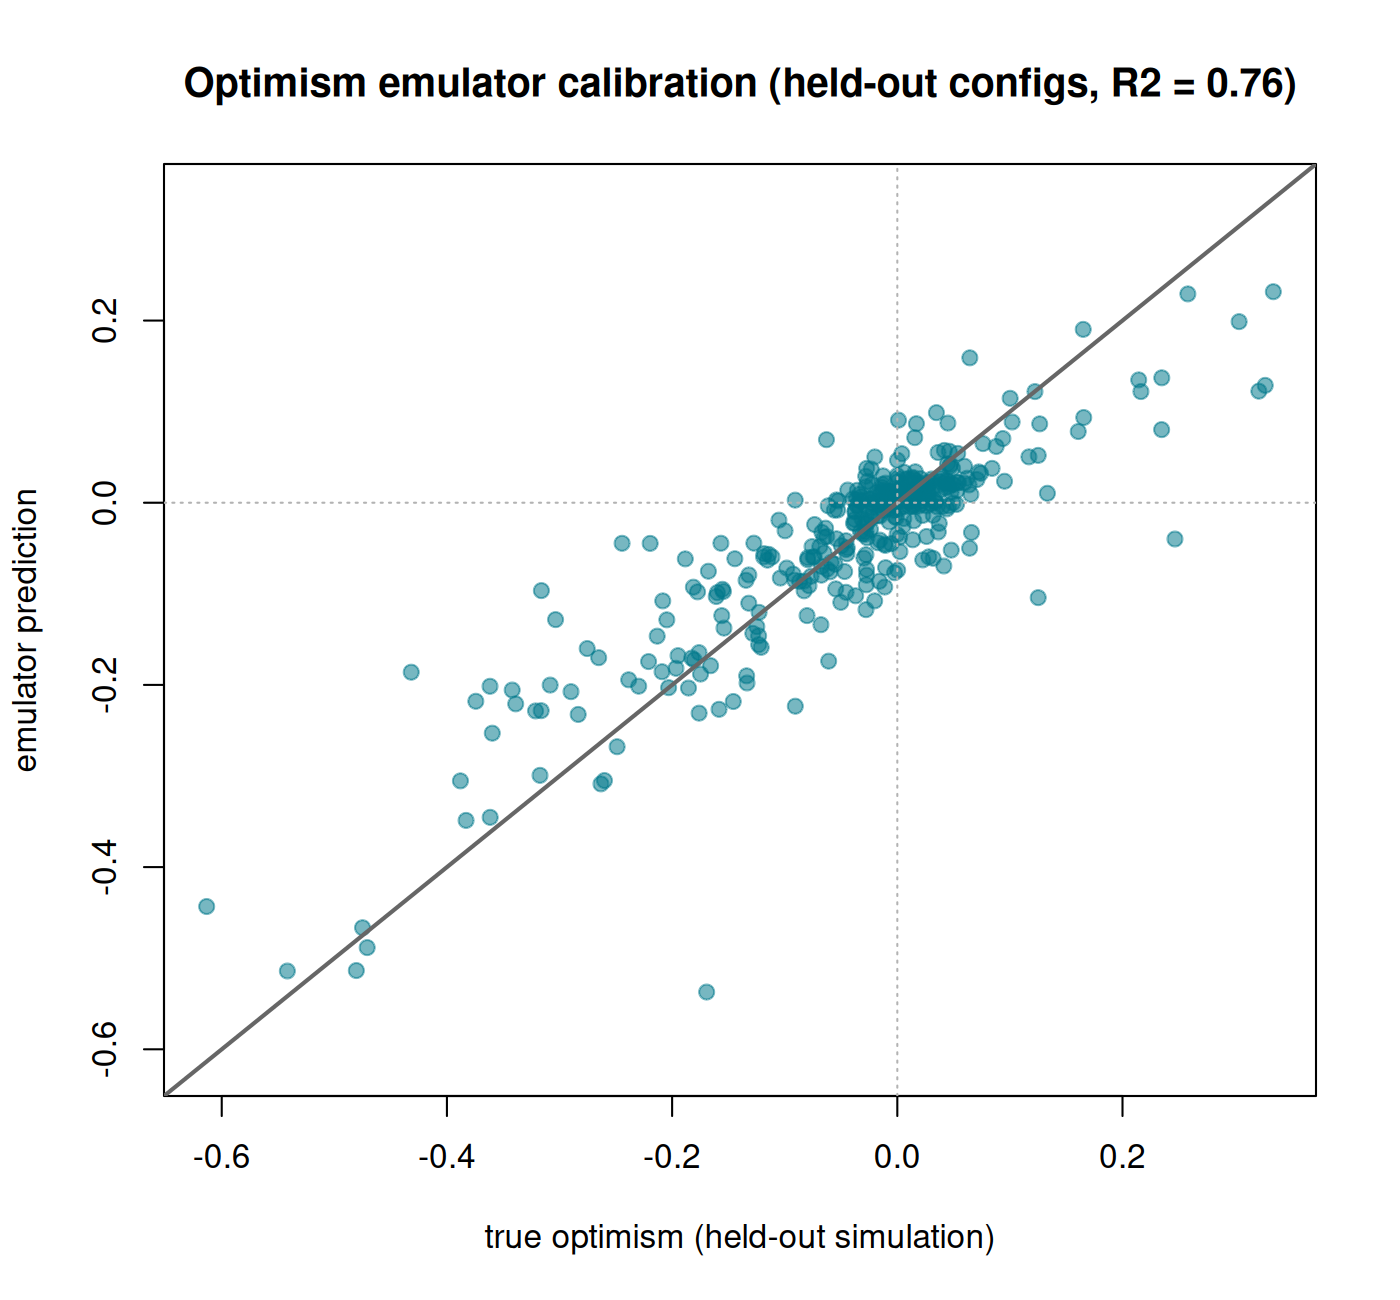
\includegraphics[width=0.74\textwidth]{figures/F1_calibration.png}
\caption{Out-of-sample calibration of the optimism emulator (held out by
configuration). Predicted vs true optimism with conformal predictive intervals;
held-out $R^2\approx 0.76$, $90\%$ interval coverage $\approx 94\%$, $97\%$ of
queries inside the area of applicability.}
\label{fig:calibration}
\end{figure}

\begin{figure}[t]
\centering
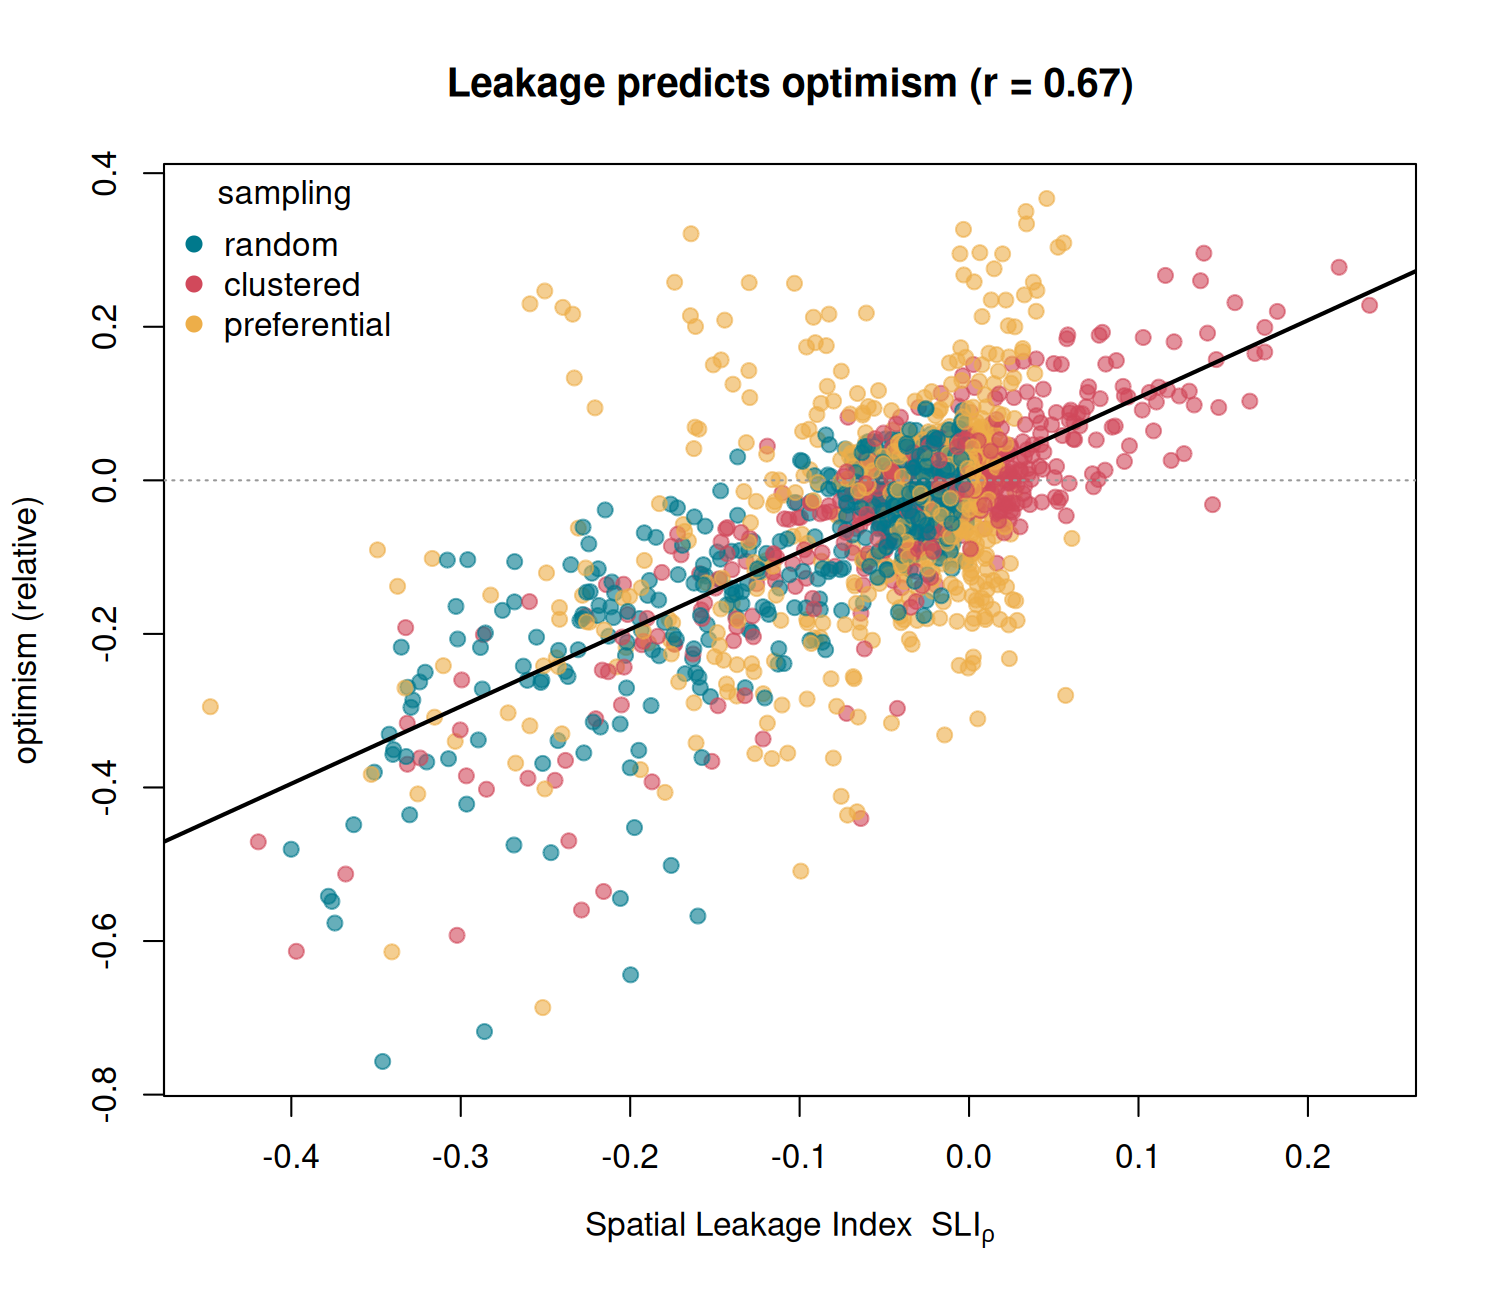
\includegraphics[width=0.74\textwidth]{figures/F2_sli_vs_optimism.png}
\caption{The Spatial Leakage Index tracks true optimism. Across the simulation grid,
$\SLIrho$ increases monotonically with measured optimism
($\cor=0.67$ empirically; $r=0.98$ against exact GP optimism), the empirical
counterpart of the closed form \eqref{eq:sliform}.}
\label{fig:sli}
\end{figure}

\begin{figure}[t]
\centering
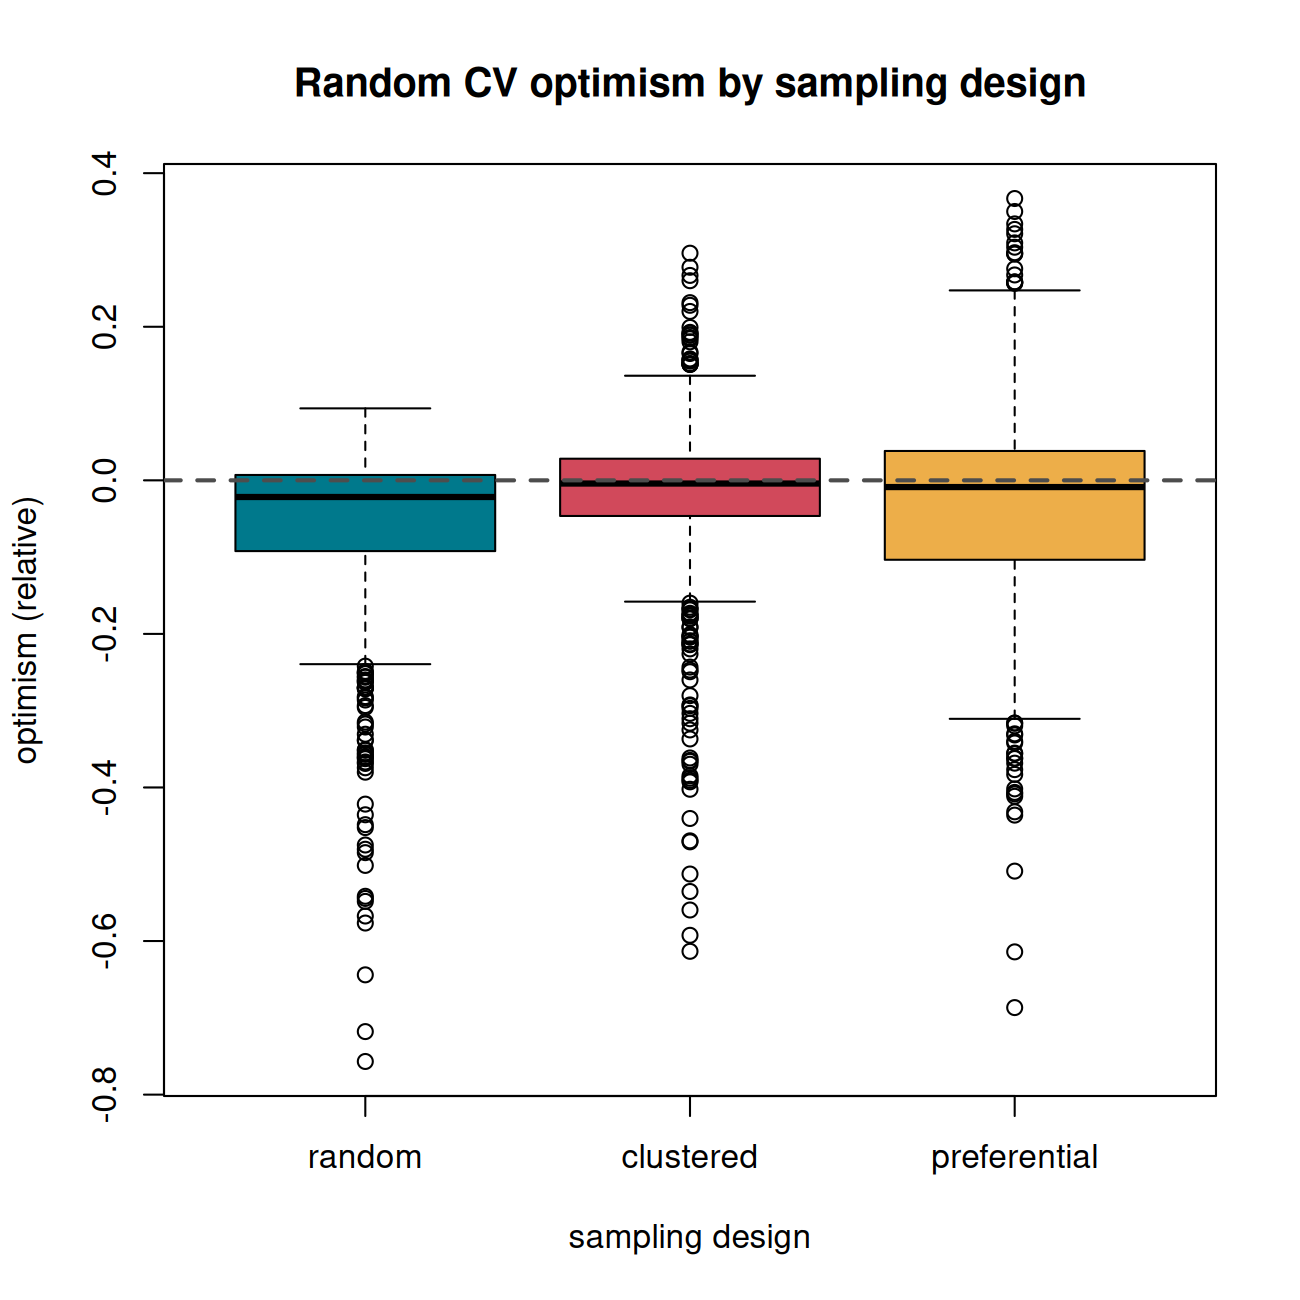
\includegraphics[width=0.74\textwidth]{figures/F3_design.png}
\caption{Reconciling Mil\`a vs Wadoux. The optimism of random CV depends on
sampling design and target: clustered/preferential designs shift random CV toward
optimism (the Mil\`a regime), whereas for probability-like samples on well-covered
targets random CV is unbiased or slightly pessimistic (the Wadoux regime). Both are
cells of one space.}
\label{fig:design}
\end{figure}

\subsection{Validation against true independent error}\label{sec:res-independent}

Simulations could be a toy, so we test on three real spatial fields (meuse
log-zinc, Paran\'a rainfall, ca20 calcium; 240 replicates), each trained on part of
the data and evaluated on a \emph{genuinely independent} held-out set, under both
extrapolation (hold out a coherent region) and interpolation (hold out an
interspersed subset) deployments. Under extrapolation, naive random 10-fold CV
\emph{understates the true independent error by a median of $36\%$}: the problem is
real and large. The target-aware SLI separates the regimes as real optimism does
(mean SLI $+0.28$ extrapolation vs $-0.01$ interpolation; mean real optimism $+0.35$
vs $-0.04$; $\cor(\SLIrho,\text{real optimism})=0.52$ across all replicates---strong
for real, noisy $n\approx 150$ data). The de-leaked estimate recovers $58\%$ of the
gap with a fixed block control and $71\%$ with the target-aware control,
reaching $0.89\times$ true independent error without ever seeing the held-out data.
The residual $29\%$ is the hardest extrapolation, where the honest answer is
area-of-applicability abstention rather than a number.

\subsection{Meta-audit: how overconfident is the field?}\label{sec:res-metaaudit}

The impact question \citep[cf.][]{ploton2020spatial}: is reported accuracy
systematically optimistic across real datasets? Using \texttt{spLeakage} as the
instrument on 16 real spatial response variables from eight public datasets (heavy
metals, soil chemistry, rainfall, elevation, ozone, malaria), with real optimism
measured by spatial region-holdout, we find reported accuracy optimistic in
\textbf{$16/16$ ($100\%$)} of cases, with median real optimism \textbf{$22\%$}
(IQR $17$--$34\%$) and $> 20\%$ in two-thirds (Figure~\ref{fig:metaaudit}).

The deeper, honest finding is that optimism has \emph{two} channels. The raw
$\SLIrho$ does \emph{not} transfer across datasets ($\cor=-0.39$)---which is the
theory, not a bug: optimism scales as $Vw^2\cdot(\cdots)$, so cross-dataset
comparison needs the signal variance the bare index omits (the SLI is a
\emph{within}-dataset predictor, validated at $\cor=0.52$ above). But even a
de-leaked estimate transfers only weakly ($+0.23$), because the smooth,
trend-dominated fields (rainfall, elevation, ozone) have the \emph{highest} real
optimism ($40$--$54\%$) yet near-zero short-range leakage: their error is the
model's inability to extrapolate a large-scale \emph{trend}, to which
autocorrelation-based diagnostics (NNDM, the SLI, the de-leak) are blind by
construction. Adding a trend-strength feature (variance explained by a quadratic
coordinate surface) recovers exactly that signal ($\cor=+0.75$, $R^2=0.56$ alone;
$R^2=0.62$ with $\lvert\SLIrho\rvert$). Real-data optimism is therefore a
two-channel phenomenon---autocorrelation (diagnosed by \texttt{detect\_leakage})
and trend extrapolation (by \texttt{trend\_strength})---and the $22\%$ median is a
\emph{lower bound} on what autocorrelation-aware tooling alone would catch.

\begin{figure}[t]
\centering
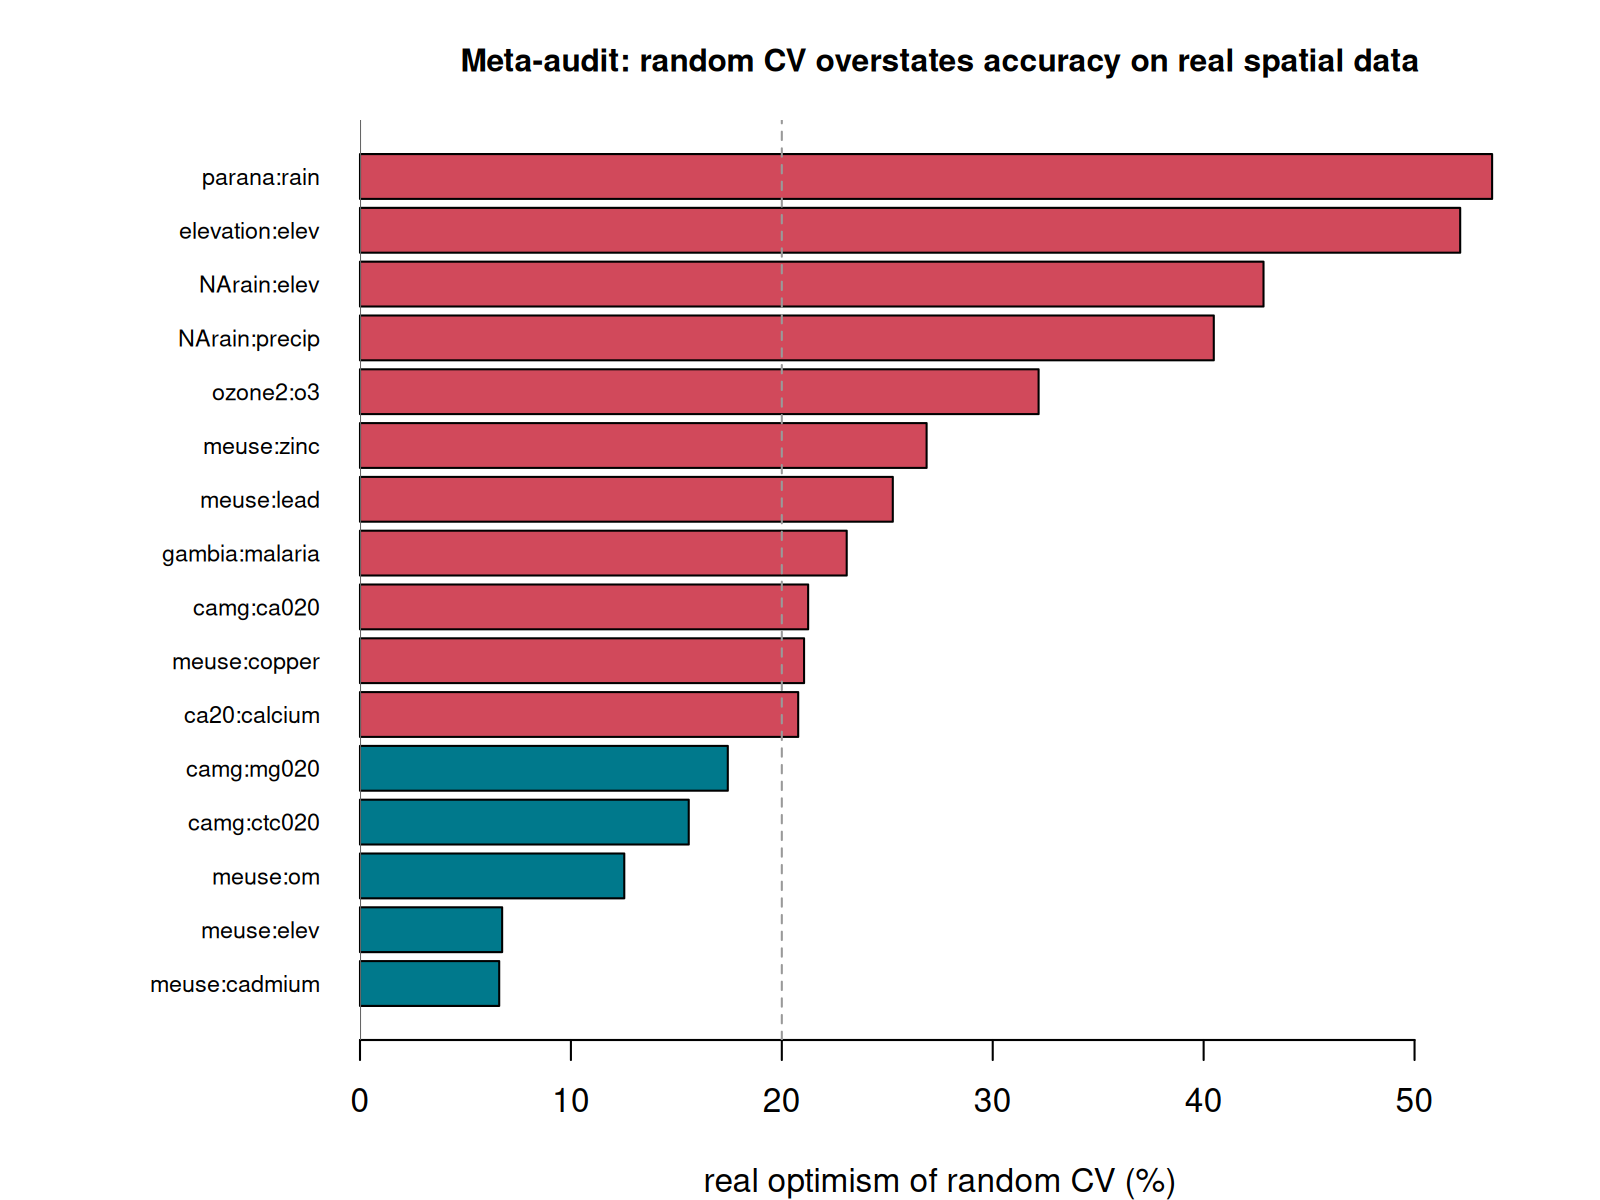
\includegraphics[width=0.78\textwidth]{figures/F4_meta_audit.png}
\caption{Meta-audit of 16 real spatial response variables. Naive random CV is
optimistic for every dataset (median $22\%$, two-thirds $>20\%$). The
trend-dominated fields (rainfall, elevation, ozone) show the largest optimism yet
the smallest short-range leakage signal---the second, trend-extrapolation channel.}
\label{fig:metaaudit}
\end{figure}

\subsection{Real-data case studies: two leakage signatures}\label{sec:res-casestudy}

Two real applications show the multi-channel audit attributing leakage to the correct
cause: a species distribution model whose optimism is genuine autocorrelation, and a
disease-prevalence map whose apparent leakage is a survey-design artefact.

\paragraph{Species distribution model.} We audit a presence/absence SDM on the
south-east Australia dataset of \citet{valavi2019blockcv} (500 records; 243 presence;
four bioclim covariates), predicting a wall-to-wall suitability map. A naive random
10-fold split validated with the Brier score is optimistic: $\SLIrho=+0.10$ (90\% CI
$+0.07,+0.14$) and the Brier score is $42\%$ better than the design-matched block
scheme (Fig.~\ref{fig:sdm}). The covariate-space channel further shows the map
\emph{extrapolates} the bioclim predictors well beyond the tested range (deployment
feature-space reach $3.73$ vs test $1.04$; signed feature leakage $+2.7$), an
area-of-applicability warning; and the grouped-location channel finds \emph{no}
co-located duplicates, so the optimism is real autocorrelation. Ranking schemes on the
data reproduces the theory's nuance: random CV optimistic ($+0.10$), buffered CV
over-corrected into pessimism ($-0.22$), block CV best matched ($-0.004$).

\begin{figure}[t]
\centering
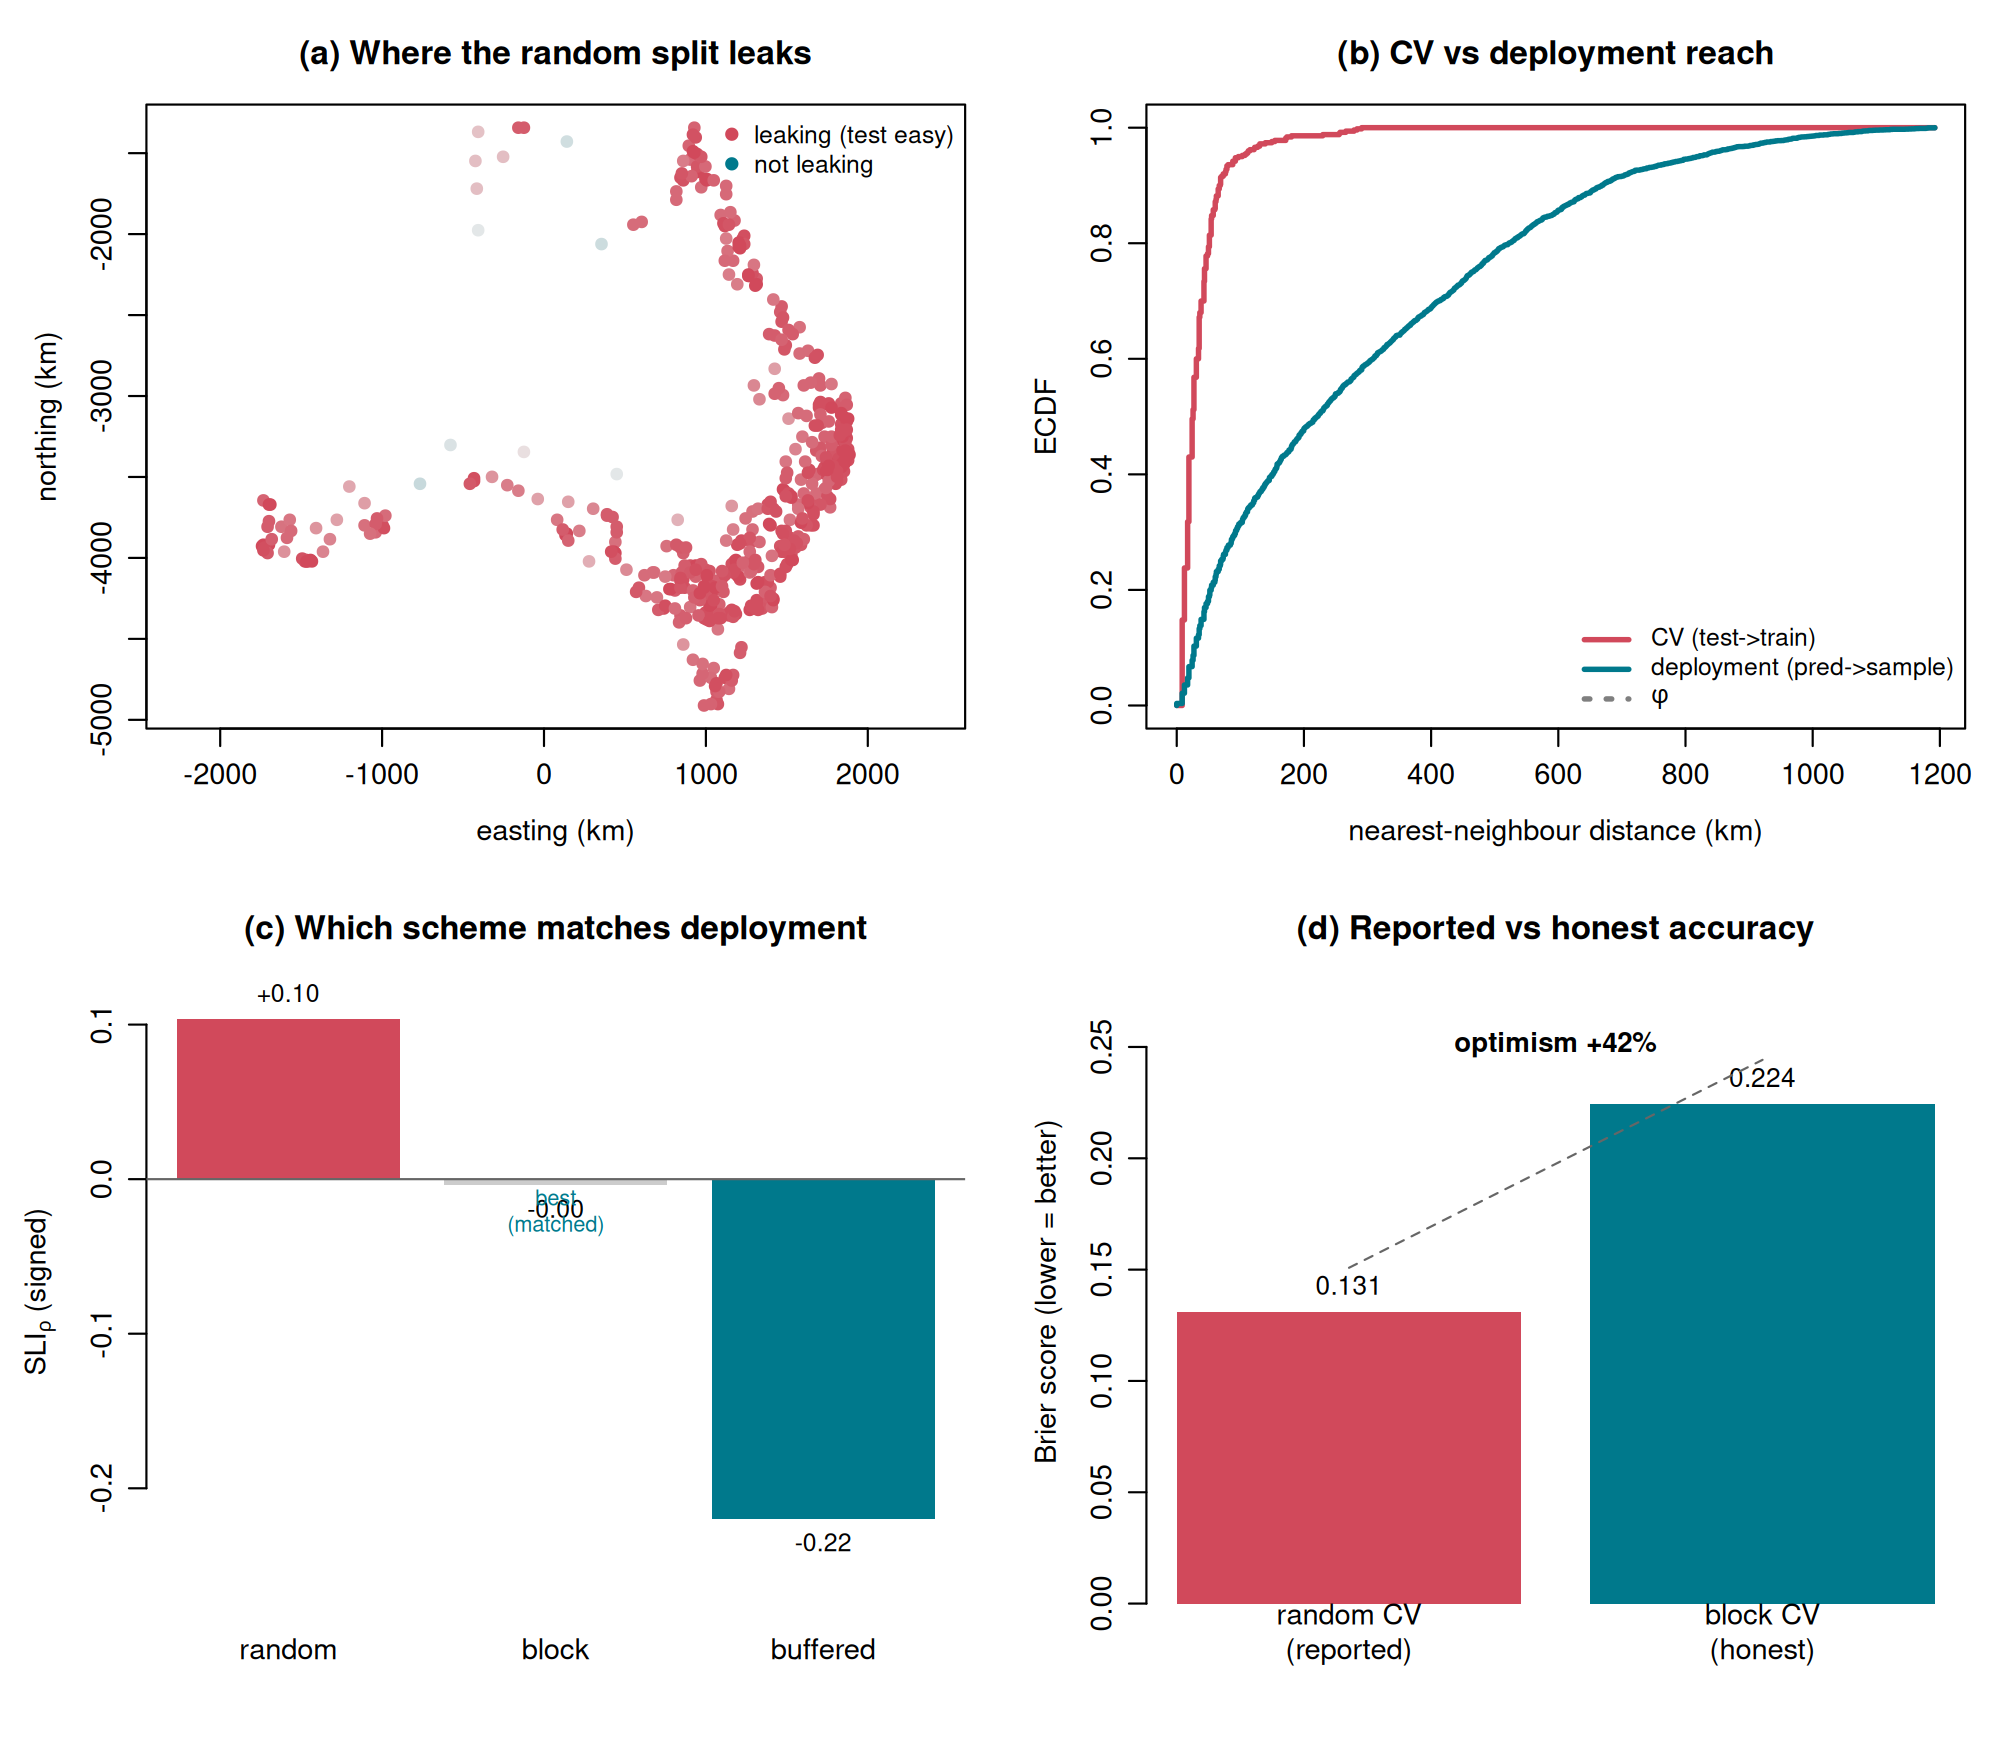
\includegraphics[width=0.92\textwidth]{figures/F5_sdm.png}
\caption{Auditing a species distribution model (south-east Australia
presence/absence; \citealp{valavi2019blockcv}). (a)~Per-point leakage map.
(b)~CV nearest-neighbour distances (red) sit far left of deployment distances
(blue)---test points are much closer to training data than the wall-to-wall map will
be ($\phi$ = variogram range). (c)~Signed SLI by scheme: random optimistic, buffered
over-corrected into pessimism, block best matched. (d)~The Brier score reported under
random CV ($0.131$) is $42\%$ better than the honest design-matched value ($0.224$).}
\label{fig:sdm}
\end{figure}

\paragraph{Malaria prevalence.} On Malaria Atlas Project \emph{Plasmodium falciparum}
prevalence \citep{weiss2019mapping} ($n=66$ geolocated surveys), a naive random
10-fold split gives $\SLIrho=+0.212$ despite a near-zero variogram signal
proportion---an apparent contradiction the package resolves. Deduplicating co-located
repeat surveys collapses $\SLIrho$ to $+0.006$; the grouped-leakage channel reports
that \textbf{$21.2\%$} of test points leak through a shared location---numerically
equal to $c_{\text{obs}}=0.212$, the two diagnostics agreeing---and
\texttt{group\_kfold()} drives it to $0\%$. Empirical optimism is a modest $+1.8\%$
(co-located records differ by year; weak signal), a textbook illustration of the
leakage-vs-optimism distinction in the wild. The emulator \emph{correctly refused} the
query ($n$ below its training envelope), demonstrating the area-of-applicability guard
on real data and deferring to the empirical route. Where the SDM's leakage was real
autocorrelation, here it is a survey-design artefact---the same audit reaching
opposite, correct verdicts.

\subsection{Designing validation surveys}\label{sec:res-design}

Finally, \texttt{design\_validation()} inverts the SLI to place validation points.
Over 120 replicates, estimating true map RMSE from a budget of 30 points, the
optimal (Neyman, inclusion-weighted) design attains \textbf{$45\%$ lower standard
deviation} than random placement for the same budget, with negligible bias---i.e.\
the same precision from 30 points that random placement needs many more to reach.
This unifies leakage diagnosis with spatial survey design.

% ===========================================================================
\section{Discussion}\label{sec:discussion}

\paragraph{What the framework settles.} The Mil\`a--Wadoux controversy is not a
disagreement about facts but about regimes. Once design, estimand and target are
declared, optimism is a well-posed, signed quantity, and the data decide which
camp's prescription applies: clustered/convenience samples make random CV
optimistic (Mil\`a); probability samples make spatial CV pessimistic (Wadoux). The
signed SLI and the optimism estimator report which regime a given analysis is in,
and the recommender prescribes accordingly---conditionally, never neutrally-but-
secretly-partisan.

\paragraph{Relationship to existing tools.} \texttt{spLeakage} is complementary to,
not competitive with, \texttt{CAST}, \texttt{blockCV}, \texttt{spatialsample} and
\texttt{mlr3spatiotempcv}. They generate corrected folds; we audit an existing split,
quantify its optimism, and---through \texttt{deleak\_estimate()}---can even correct a
published number without the original model. The reduction $\lvert A\rvert=W$ makes
the bridge to NNDM explicit.

\paragraph{Scope and limitations.} The closed-form theory is the Gaussian backbone:
the single-NN approximation underestimates magnitude for dense training (corrected
by a $\approx 1.6\times$ multi-neighbour factor or the exact $c_0^\top\Sigma^{-1}
c_0$); non-Gaussian responses and sub-optimal learners (RF, GAM) are handled
empirically by the emulator, for which the GP gives the envelope (real learners'
explained variance is no larger than kriging's). The emulator is honest about its own
extrapolation through the area-of-applicability guard, and abstains rather than
guess---as it did on the Nigeria query. The most important open finding is the
\emph{second channel}: a large-scale trend-extrapolation component of optimism that
all autocorrelation-based diagnostics (including ours) miss, now measurable via
\texttt{trend\_strength} but deserving a fully trend/covariate-aware optimism model.
Finally, design-basedness must be elicited; no geometric test can certify a sample
as a probability sample, so the recommender is decision \emph{support}, not
automation.

\paragraph{Outlook.} The distribution-shift framing \eqref{eq:wbound} points toward
model-agnostic optimism bounds beyond the GP (importance weighting,
integral-probability metrics), broadening the audience from spatial statistics to
machine learning. Coupling the autocorrelation and trend channels into a single
optimism model, and extending the emulator's generators to spatial GLMMs with
covariate trends, are the natural next steps.

\paragraph{Conclusion.} Reported accuracy for spatial maps is, across a wide range
of real datasets, materially and systematically optimistic. \texttt{spLeakage}
makes that optimism well-posed, measurable, signed, correctable and---through
validation design---cheaper to pin down, while reconciling a controversy that has
left practitioners without clear guidance. By auditing rather than generating folds,
it adds a missing diagnostic layer to the spatial-prediction workflow.

% ===========================================================================
\section*{Data and code availability}
The \texttt{spLeakage} package, including all analysis scripts in
\texttt{data-raw/} that reproduce the results in Section~\ref{sec:results}, is
openly available at \url{https://github.com/olatunjijohnson/spLeakage} under an MIT
licence. All datasets used are public (the south-east Australia presence/absence SDM
data and bioclim covariates via \texttt{blockCV}; Malaria Atlas Project via the
\texttt{malariaAtlas} R package; \texttt{meuse}, \texttt{ca20}, Paran\'a and the
remaining meta-audit fields via \texttt{sp}, \texttt{geoR} and \texttt{gstat}).

\section*{Acknowledgements}
The author thanks the developers of the spatial cross-validation ecosystem
(\texttt{CAST}, \texttt{blockCV}, \texttt{spatialsample},
\texttt{mlr3spatiotempcv}) whose work this package builds upon and audits.

\section*{Conflict of interest}
The author declares no conflict of interest.

\bibliography{refs}

\end{document}
